\documentclass[tikz,border=2pt]{standalone}
\usepackage{lmodern}
\usepackage{xcolor}
\usetikzlibrary{arrows.meta}
\definecolor{paletteGreen}{HTML}{2A6F62}
\definecolor{paletteOrange}{HTML}{D96C3D}

\begin{document}
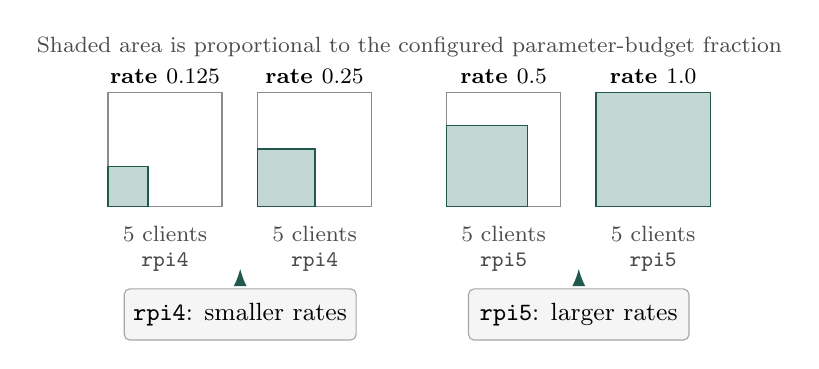
\begin{tikzpicture}[
  font=\small,
  fullmodel/.style={draw=black!45, line width=0.45pt, fill=white},
  active/.style={draw=paletteGreen!80!black, line width=0.5pt, fill=paletteGreen!28},
  device/.style={draw=black!35, rounded corners=2pt, fill=black!4, align=center, minimum height=0.65cm},
  note/.style={font=\footnotesize, align=center, text=black!70}
]
\def\fullside{1.45}
\newcommand{\ratecard}[5]{%
  \begin{scope}[shift={(#1,0)}]
    \node[font=\footnotesize\bfseries] at (0.725,2.08) {#2};
    \draw[fullmodel] (0,0.42) rectangle ++(\fullside,\fullside);
    \draw[active] (0,0.42) rectangle ++(#3,#3);
    \node[note] at (0.725,0.08) {#4};
    \node[note] at (0.725,-0.28) {#5};
  \end{scope}
}
\ratecard{0.0}{rate \(0.125\)}{0.51}{\(5\) clients}{\texttt{rpi4}}
\ratecard{1.9}{rate \(0.25\)}{0.73}{\(5\) clients}{\texttt{rpi4}}
\ratecard{4.3}{rate \(0.5\)}{1.03}{\(5\) clients}{\texttt{rpi5}}
\ratecard{6.2}{rate \(1.0\)}{1.45}{\(5\) clients}{\texttt{rpi5}}

\node[device, minimum width=2.8cm] at (1.68,-0.95) {\texttt{rpi4}: smaller rates};
\node[device, minimum width=2.8cm] at (5.98,-0.95) {\texttt{rpi5}: larger rates};
\draw[-{Latex[length=2.2mm]}, paletteGreen!80!black, line width=0.5pt] (1.68,-0.58) -- (1.68,-0.37);
\draw[-{Latex[length=2.2mm]}, paletteGreen!80!black, line width=0.5pt] (5.98,-0.58) -- (5.98,-0.37);
\node[note] at (3.83,2.45) {Shaded area is proportional to the configured parameter-budget fraction};
\end{tikzpicture}
\end{document}
